\chapter{Development with Certainty}

In this chapter, we elaborate on deterministic analysis of computer systems. The
techniques that we discuss here do not take uncertainty into account. However,
these techniques provide a solid foundation for those that do as we shall
describe in the following chapter, \cref{development-uncertainty}.

\section{Introduction}

Due to the rapidly increasing power densities, temperature has evolved into an
acute concern of computer-system designs, and temperature analysis has become an
essential component of design workflows. With this in mind, we focus our
attention on this analysis and its accompanying disciplines.

There are two types of temperature analysis: \one~transient analysis and
\two~steady-state analysis. The first delivers the temperature that the system
at hand transitions over within an arbitrary time interval staring from
arbitrary initial conditions when it is exposed to an arbitrary, both spatially
and temporally, power distribution. The second delivers the temperature that the
system attains and retains once it has reached a thermal equilibrium under a
power distribution that is spatially arbitrary but temporally constant or
repeating.

Steady-state analysis can be further classified into two categories, which have
already been alluded to: \one~static analysis and \two~dynamic analysis. The
first is concerned with temporally constant power distributions, that is, with
those that do not change over time. In this case, temperature distributions do
not change over time either. The second is concerned with temporary arbitrary
power distributions that are periodic, that is, with those that repeat with
certain periods. In this case, temperature distributions change over time with
the same periods as the corresponding repeating power distributions.

The agenda for the rest of this chapter is as follows. In
\sref{temperature-analysis}, we present the general model that is used in all
the three aforementioned types of temperature analysis. Transient analysis,
static steady-state analysis, and dynamic steady-state analysis are then
discussed separately in \sref{transient-analysis},
\sref{static-steady-state-analysis}, and \sref{dynamic-steady-state-analysis},
respectively. Lastly, the importance of the last in the context of reliability
optimization is covered in \sref{reliability-optimization}.

\section{Temperature Analysis}
\slab{temperature-analysis}

Temperature analysis of electronic systems is chiefly based on the duality
between the transfer of heat and the transfer of electric charge
\cite{kreith2000}. The core idea is to construct a so-called thermal \up{RC}
circuit for the system under consideration \cite{skadron2003}. Such a circuit is
a collection of thermal nodes that are characterized by thermal capacitances and
connected with each other via thermal resistances. The circuit is to capture the
relevant physical structure and thermal properties of the system and, thereby,
to model the system's thermal dynamics.

Consider now a generic electronic system that consists of \nc processing
elements and is equipped with a thermal package. The processing elements are the
active components of the system, that is, those that consume power. The thermal
package is the cooling equipment of the system including any passive components,
that is, those that do not consume power. Processing elements can be identified
at different levels of granularity; for instance, a processing element can be a
whole \up{SoC}, an individual \up{CPU}, or even an \up{ALU}. A thermal \up{RC}
circuit can also be constructed at different levels of granularity, which
primarily refers to the number thermal nodes, denoted by \nn in what follows,
and their placement. It should be understood that the chosen granularity level
has a profound impact on the accuracy of the subsequent temperature analysis.

\begin{figure*}
  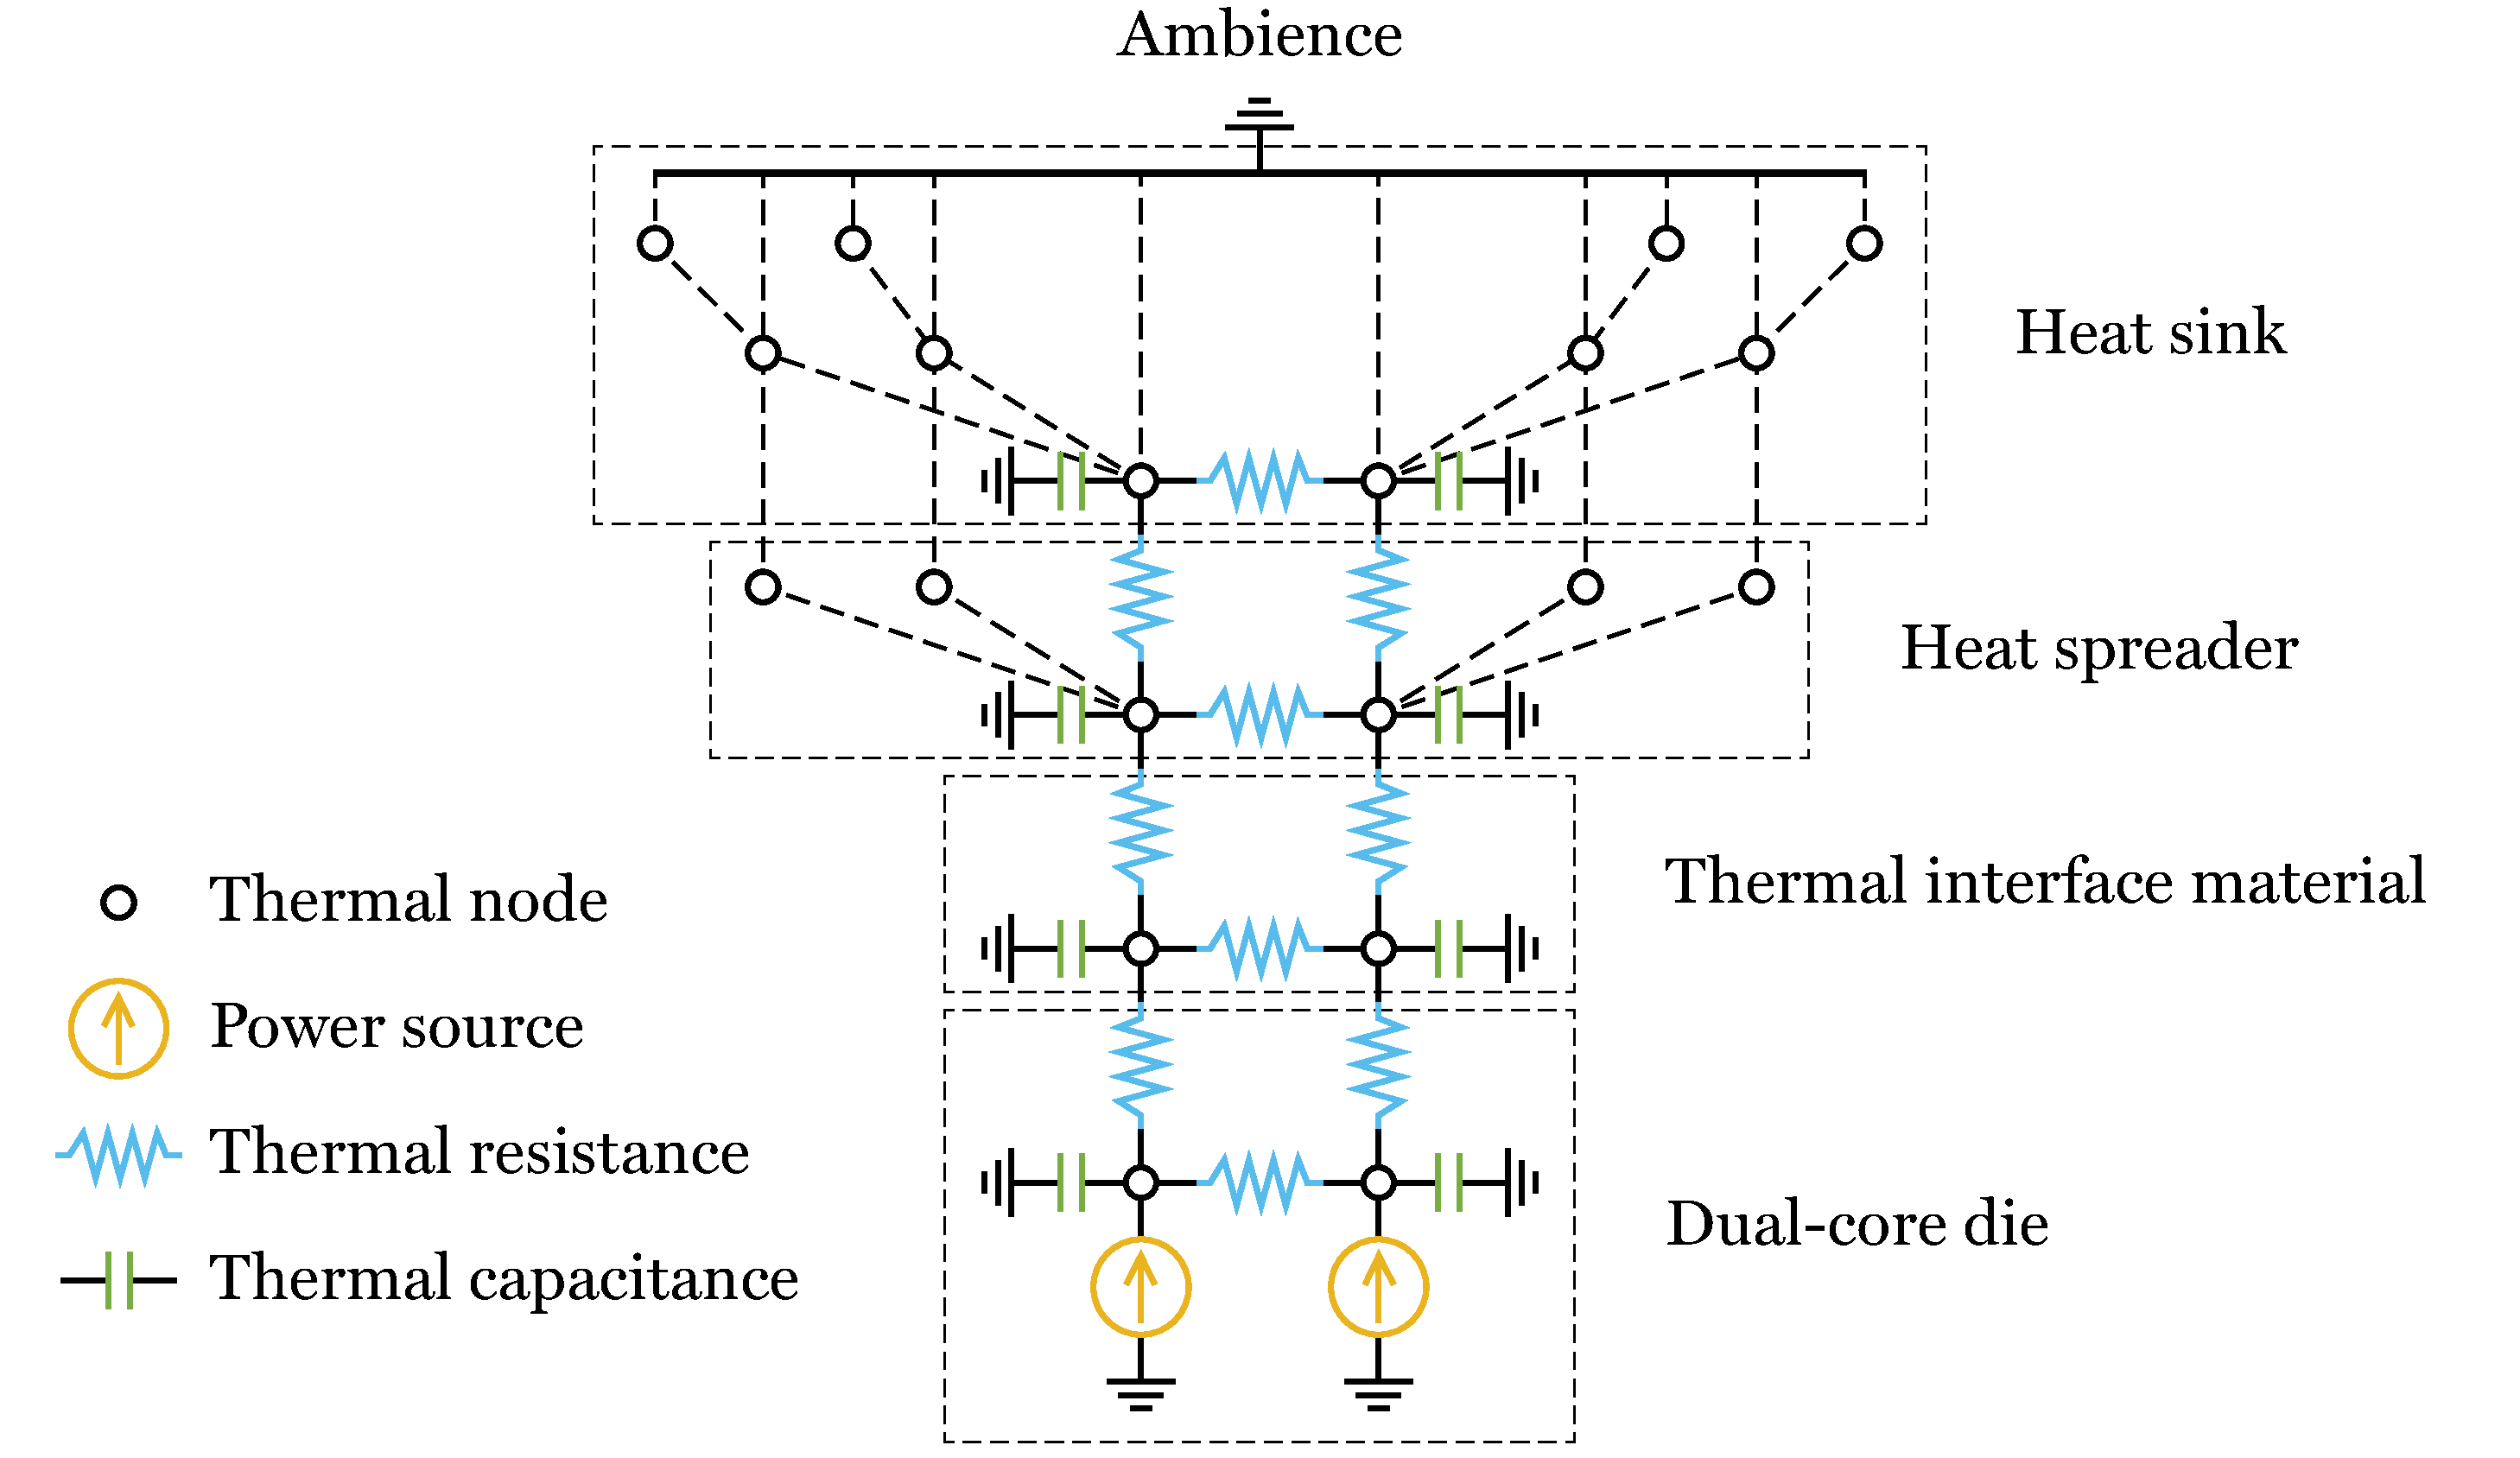
\includegraphics[width=1.0\textwidth]{include/assets/figures/circuit.pdf}
  \caption{Example of a thermal \up{RC} circuit.}
  \flab{circuit}
\end{figure*}

In order to give a better intuition about thermal \up{RC} circuits,
\fref{circuit} depicts a simplified example of a circuit constructed for a
hypothetical dual-core chip equipped with a thermal package composed of a
thermal interface material, heat spreader, and heat sink. Each of the $\nc$
processing elements is represented by one thermal node, and the thermal
interface material, heat spreader, and heat sink are captured by \nc, $\nc + 4$,
and $\nc + 8$ nodes, respectively. Thus, the total number of thermal nodes \nn
is $4 \times \nc + 12$. In this example, $\nc = 2$ and $\nn = 20$. The general
construction principle described above is the one presented in
\cite{skadron2003, huang2008}, and it is also the one used throughout this
thesis.

Suppose now that an adequate thermal \up{RC} circuit has been constructed for
the considered electronic system. Regardless of the structure of the circuit,
the thermal dynamics of the circuit (and the electronic system) are governed by
the following system of $\nn$ differential and $\nc$ algebraic equations:
\begin{equation} \elab{temperature-model-original}
  \begin{cases}
    & \m{C} \frac{d\vs(t)}{dt} + \m{G} \vs(t) = \m{M} \vp(t) \\
    & \vq(t) = \m{W} \vs(t) + \vq_\ambient
  \end{cases}.
\end{equation}
In \eref{temperature-model-original}, $\vq \in \real^\nc$, $\vq_\ambient \in
\real^\nc$, and $\vp \in \real^\nc$ are vectors of the operating temperature,
ambient temperature, and power dissipation of the processing elements,
respectively. Furthermore, $\vs \in \real^\nn$ captures the relative temperature
of the thermal nodes, and $\m{C} \in \real^{\nn \times \nn}$ and $\m{G} \in
\real^{\nn \times \nn}$ are a diagonal matrix of the thermal capacitance and a
symmetric and positive-definite matrix of the thermal conductance, respectively.
Lastly, $\m{M} \in \real^{\nn \times \nc}$ is a matrix that maps the power of
the processing elements onto the thermal nodes, and $\m{W} \in \real^{\nc \times
\nn}$ is a matrix that maps the temperature of the thermal nodes onto the
processing elements. Without loss of generality, $\m{M}$ is assumed to be a
rectangular diagonal matrix whose diagonal elements are equal to unity, and
$\m{W} = \m{M}^\transpose$.

\section{Transient Temperature Analysis}
\slab{transient-analysis}

The parameters of the die and thermal package, used throughout this paper, are
given in \tref{parameters}.

\begin{table}[b]
  \vspace{15pt}
  \caption{Parameters of the die and package.}
  \tlab{parameters}
  \centering
  \begin{tabular}{|l|r|}
    \hline
    Parameter & Value \\
    \hline
    \hline
    Ambient temperature                   &   27 ${}^\circ C$ \\
    Convection capacitance                & 140.4 J/K \\
    Convection resistance                 & 0.1 K/W \\
    Die thickness                         & 0.15 $mm$ \\
    Thermal interface material thickness  & 0.02 $mm$ \\
    Heat spreader side                    &   20 $mm$ \\
    Heat spreader thickness               &    1 $mm$ \\
    Heat sink side                        &   30 $mm$ \\
    Heat sink thickness                   &   15 $mm$ \\
    \hline
  \end{tabular}
\end{table}

\section{Static Steady-State Temperature Analysis}
\slab{static-steady-state-analysis}

\section{Dynamic Steady-State Temperature Analysis}
\slab{dynamic-steady-state-analysis}

The static steady-state temperature produced by static steady-state analysis is
an approximation of the system's thermal behavior with limited applicability. It
assumes that, eventually, the system will function at one constant temperature
at each spatial location. This, however, is very often not the case in reality.
In the context of a variable power profile applied periodically, the circuit
will not reach a constant steady-state temperature but a steady state in which
temperature is varying according to a certain periodic pattern. This pattern is
captured by the steady-state dynamic temperature profile (SSDTP).

However, temperature analysis time with HotSpot, or other similar approaches, is
too long to be used inside a temperature-aware system-level optimization loop.
The long thermal simulation time can severely limit the efficiency of the design
space exploration. There has been some work on establishing fast system-level
temperature analysis techniques. They also build on the duality between heat
transfer and electrical phenomena and are based on restrictive assumptions in
order to simplify the model. The approaches proposed in \cite{rai2011, bao2010},
for example, are strictly restricted to monocore systems. The method described
in \cite{rao2009} is restricted to homogeneous platforms and to applications in
which the execution time of individual tasks is long, comparable with the
thermal time constant of the package (in the order of 100 $s$).

In the case of applications that exhibit periodic or close to periodic behavior
(or which are characterized by several operation modes, each of which exhibits a
periodic behavior), the SSDTP is of particular importance for system design. Any
design optimization has to be performed such that the efficiency and reliability
of the system are maximized considering not a very short transient time interval
at system start (or mode setup) but the context in which the system functions
over a long period of time.

A typical design task, for which the SSDTP is of central importance, is
temperature-aware reliability optimization. The impact of temperature on the
lifetime of electronic circuits is well-known \cite{srinivasan2004, coskun2006,
xiang2010, jedec2010}. The failure mechanisms commonly considered are
electromigration, time-dependent dielectric breakdown, and thermal cycling,
which are directly driven by the temperature \cite{jedec2010}. What is important
in this context is that not only average and maximum temperature, but also the
amplitude and frequency of temperature oscillations, have a huge impact on the
overall lifetime of the chip. Thus, efficient reliability optimization depends
on the availability of the actual SSDTP.

Two approaches have been applied in the literature in order to obtain the SSDTP,
as a prerequisite for reliability optimization. An approximate SSDTP can be
produced by running a temperature simulator over one or more successive periods
of the application until one can assume that a sufficient approximation of the
thermal steady state has been reached \cite{srinivasan2004}. Such an approach is
both time consuming and potentially inaccurate. A very rough but fast
approximation of the SSDTP is proposed in \cite{huang2009}. It constructs a
stepwise temperature curve where each step corresponds to the static
steady-state temperature that would be reached if a certain constant power was
applied for a sufficiently long time. In \sref{hotspot-solution} we will further
elaborate on these two state of the art solutions. As our experiments show, they
are too slow and/or too inaccurate in order to efficiently be used inside a
temperature-aware system-level optimization loop for, e.g., reliability
optimization.

In this paper we consider multiprocessor systems running applications exhibiting
a power profile that can be considered periodic. Our contribution is twofold.
First, we propose an approach that is both accurate and fast, for SSDTP
calculation. Second, we show how our approach makes it possible to efficiently
perform reliability optimization, based on the thermal cycling (TC) failure
mechanism. More exactly, we propose a temperature-aware task mapping and
scheduling technique that addresses the TC ageing effect. Experiments
demonstrate the superiority of the proposed techniques, compared to the state of
the art.

\subsection{Problem Formulation}

Consider a multicore system that consists of $N_p$ processing elements $\Pi = \{
\pi_i: i = \range{0}{N_p - 1} \}$ and executes a periodic application with a
period $\tau$. We construct an equivalent RC thermal circuit of the system that
contains $N_n$ thermal nodes. The dynamic power profile of the system is sampled
into $N_s$ time intervals of duration $\Delta t$, called sampling interval, in
such a way that the dynamic power dissipation and temperature of each node are
assumed to be constant within an interval. The discrete dynamic power profile is
defined as the following:
\[
  \mathbb{P}_\text{dyn} := \{ P_{ij}: \: i = \range{0}{N_s - 1}; \: j = \range{0}{N_n - 1} \}
\]
where $P_{ij}$ is the dynamic power dissipation during the $i$th time interval
of the $j$th thermal node. After the steady state is reached, the corresponding
temperature profile becomes periodic and is defined as:
\[
  \mathbb{T} := \{ T_{ij}: \: i = \range{0}{N_s - 1}; \: j = \range{0}{N_n - 1} \}
\]
where $T_{ij}$ is the temperature of the $j$th node in the $i$th time interval.
The profile is called the steady-state dynamic temperature profile (SSDTP).

Given:
\begin{itemize}

\item A multicore system with a set of processing elements $\Pi$ executing a
periodic application.

\item The discrete dynamic power profile $\mathbb{P}_\text{dyn}$ of the
system\footnote{Power dissipation of inactive nodes, i.e., the nodes that belong
to the thermal package, is zero.} with the sampling interval $\Delta t$.

\item The floorplan of the chip corresponding to the level of details at which
the thermal modeling is performed.

\item The configuration of the thermal package, i.e., dimensions of the thermal
interface material, heat spreader, and heat sink.

\item The thermal parameters of the die and package, e.g., the thermal
conductivity and thermal capacitance.

\end{itemize}

Find:
\begin{itemize}

\item The corresponding periodic temperature profile $\mathbb{T}$ of the system
when the steady state is reached.

\end{itemize}
Reasonable requirements for a solution are speed and accuracy, since the
temperature analysis is often a part of an intensive optimization procedure
where the SSDTP is to be computed thousands of times. Such a problem is
described in \sref{reliability-optimization}.

\subsection{State of the Art Solutions}
\slab{hotspot-solution}

\subsubsection{Iterative Simulation}
\slab{hotspot-iterative-solution}

A rough approximation of the SSDTP can be obtained by running a temperature
simulation over successive periods of the application until it can be assumed
that the system has reached the thermal steady state. The simulator performs the
transient temperature analysis where the common approach is to solve
\eref{temperature-model-original} numerically, for instance, using the
fourth-order Runge-Kutta method \cite{press2007}.

HotSpot \cite{skadron2003}, an architecture and system-level model and
simulator, is the state of the art choice for system-level temperature analysis,
as in \cite{srinivasan2004, liao2005, coskun2006, liu2007, huang2009, xiang2010,
thiele2011}.

The number of iterations required to reach the SSDTP depends on the thermal
characteristics of the system. In order to illustrate this aspect, we have
considered an application with the period of 0.5 $s$ running on five
hypothetical platforms with core areas between 1 and 25 $mm^2$. The
configuration of the die and thermal package can be found in the appendix
(\tref{parameters}). We have run the temperature simulation with HotSpot
\cite{skadron2003} for 50 successive periods. The temperature profile in each
period has been compared with the actual SSDTP, obtained with our analytical
approach (\sref{condensed-equation}), and the normalized root mean square error
(NRMSE) has been calculated. The result is shown in \fref{hotspot-error}. It can
be observed that the number of successive periods over which the temperature
simulation has to be performed, in order to achieve a satisfactory level of
accuracy, is significant for the majority of configurations. For a 9 $mm^2$ die,
for example, after 15 iterations, the NRMSE is still close to 20\%. This leads
to large computation times, making it difficult to apply the technique inside an
intensive optimization loop.

\subsubsection{Steady-State Approximation (SSA)}
\slab{steady-state-approximation}

An approximation of the SSDTP has been proposed in \cite{huang2009}. Instead of
solving the system of equations in \eref{temperature-model-original}, it is
assumed that during each time interval $\Delta t_i$, in which the power is
constant, the system stays in its steady state. The derivative $d\v{T}/dt = 0$
and temperature can be calculated as $\v{T}_i = \m{G}^{-1} \v{P}_i$. The result
is a stepwise temperature curve where each step corresponds to the steady-state
temperature $\v{T}_i$ that would be reached if the constant power $\v{P}_i$ was
applied for a sufficiently long time.

An example of such an approximation (SSA) along with the corresponding SSDTP for
an application with 10 tasks and period of 0.1 $s$ is given in
\fref{steady-state-approximation}. The die area is 25 $mm^2$, the configuration
of the chip is the same as in \tref{parameters}. The reduced accuracy of the SSA
is due to the mismatch between the actual temperature within each interval
$\Delta t_i$ and the hypothetical steady-state temperature. The inaccuracy
depends on the thermal characteristics of the respective platform and on the
application itself. To illustrate this, we have generated five applications with
periods between 0.01 and 1~$s$ and computed approximated SSDTPs using the SSA
for die areas between 1 and 25 $mm^2$. The NRMSE relative to the correct SSDTP
is shown in \fref{steady-state-error}. It can be seen that, e.g., for a die area
of 10 $mm^2$ and a period of $100~ms$ the NRMSE with the SSA is close to 40\%.

\subsection{Proposed Technique}
\slab{condensed-equation}

\subsection{Analytical Solution}
\slab{analytical-solution}

As shown in \sref{hotspot-solution}, the state of the art solutions either
produce inaccurate and, in many cases, completely useless results, or they are
unacceptably slow. In this section we eliminate the first problem by obtaining
an analytical solution for the SSDTP and tackle the second one in
\sref{condensed-equation} where a fast solution technique is proposed.

In the following explanation, without loss of generality, we assume $\v{T}(t)
\equiv \v{T}(t) - \v{T}_\ambient$. Let the power consumption vector $\v{P}(t)$
be constant and equal to $\v{P}$; then the system given by
\eref{temperature-model-original} is a system of ordinary differential equations
(ODE) with the following solution:
\begin{equation} \elab{solution}
  \v{T}(t) = e^{\m{A} t} \; \v{T}_0 + \m{A}^{-1} (e^{\m{A} t} - \m{I}) \; \m{C}^{-1} \v{P}
\end{equation}
where $\m{A} = -\m{C}^{-1} \: \m{G}$, $\v{T}_0$ is the initial temperature and
$\m{I}$ is the identity matrix. Therefore, given a discrete power profile, the
corresponding temperature profile can be found using the following recurrence:
\begin{equation} \elab{recurrent-system}
  \v{T}_{i+1} = \m{K}_i \: \v{T}_i + \m{B}_i \: \v{P}_i
\end{equation}
where $\m{K}_i = e^{\m{A} \Delta t_i}$ and $\m{B}_i = \m{A}^{-1}(e^{\m{A} \Delta
t_i} - \m{I})\m{C}^{-1}$. The approach can be used to perform the TTA as it is
discussed in the appendix (\sref{tta-analytical}).

For the SSDTA calculation the following system of linear equations can be
derived from \eref{recurrent-system}:
\[
  \begin{cases}
    \m{K}_0 \: \v{T}_0 - \v{T}_1 & = -\m{B}_0 \: \v{P}_0 \\
    ... \\
    -\v{T}_0 + \m{K}_{N_s - 1} \: \v{T}_{N_s - 1} & = -\m{B}_{N_s - 1} \: \v{P}_{N_s - 1}
  \end{cases}
\]
where the last equation enforces the boundary condition, the equality of
temperature values on both ends of the period:
\begin{equation} \elab{boundary-condition}
  \v{T}_0 = \v{T}_{N_s}
\end{equation}
To get the whole picture, the system can be written as:
\begin{equation} \elab{system}
\resizebox{0.9\linewidth}{!}{
  $\underbrace{\left[
    \begin{array}{ccccc}
      \m{K}_0 & -\m{I} & 0 & \cdots & 0 \\
      0 & \m{K}_1 & -\m{I} &  & \vdots \\
      \vdots &  & \ddots & -\m{I} & 0 \\
      0 &  &  & \m{K}_{N_s - 2} & -\m{I} \\
      -\m{I} & 0 & \cdots & 0 & \m{K}_{N_s - 1}
    \end{array}
  \right]}_{\displaystyle \mathbb{A}} \underbrace{\left[
    \begin{array}{c}
      \v{T}_0 \\
      \\
      \vdots \\
      \\
      \v{T}_{N_s - 1}
    \end{array}
  \right]}_{\displaystyle \mathbb{X}} = \underbrace{\left[
    \begin{array}{c}
      -\m{B}_0 \: \v{P}_0 \\
      \\
      \vdots \\
      \\
      -\m{B}_{N_s - 1} \: \v{P}_{N_s - 1}
    \end{array}
  \right]}_{\displaystyle \mathbb{B}}$
}
\end{equation}
where $\mathbb{A}$ is a $N_n N_s \times N_n N_s$ matrix, $\mathbb{X}$ and
$\mathbb{B}$ are vectors with $N_n N_s$ elements. It can be seen that we have
obtained a regular system of linear equations. Straight-forward techniques to
solve it and their disadvantages are further discussed in the appendix
(\sref{straight-forward}).

In this section we propose a fast approach to solve the system in \eref{system}.
The approach consists of an auxiliary transformation (\sref{ce-auxiliary}) and
the actual solution (\sref{ce-solution}).

The major problem with straight-forward techniques (see \eref{straight-forward})
is that (1) the sparseness of the matrix is not taken into account and/or (2)
its specific structure is totally ignored, resulting in inefficiency and
inaccuracy of the computations. Using direct dense and sparse solvers, for
example, requires a computation time proportional to $N_n^3 N_s^3$
\cite{press2007}. Our proposed technique considers both features and delivers
solutions in time proportional to $N_s N_n^3$ while operating only on a few $N_n
\times N_n$ matrices. It is important that the dependency on $N_s$ (the number
of steps in the power profile), which is by far dominating ($N_s \gg N_n$), is
linear.

Observing the structure of the matrix in \eref{system}, non-zero elements are
located only on the block diagonal, on one subdiagonal just above the block
diagonal, and on one subdiagonal in the left bottom corner. The block diagonal
is composed of $N_n \times N_n$ matrices while all elements of the subdiagonals
are equal to $-1$. Linear systems with the same structure arise in boundary
value problems for ODEs where a technique to solve them is to form a so-called
condensed equation (CE), or condensed system \cite{stoer2002}.

\subsection{Auxiliary Transformation}
\slab{ce-auxiliary}

The analytical solution in \eref{solution} includes two computationally
expensive operations, namely the matrix exponential and inverse involving
\mbox{$\m{A} = - \m{C}^{-1} \: \m{G}$}, which is an arbitrary square matrix. It
is preferable to have a symmetric matrix to perform these computations, since
for a real symmetric matrix $\m{M}$ the following eigenvalue decomposition with
independent eigenvectors holds \cite{press2007}:
\begin{equation} \elab{eigenvalue-decomposition}
  \m{M} = \m{U} \m{\Lambda} \m{U}^\v{T}
\end{equation}
where $\m{U}$ is a square matrix of the eigenvectors, $\m{U}^T$ is the transpose
of $\m{U}$, and $\m{\Lambda}$ is a diagonal matrix of the eigenvalues
$\lambda_i$ of $\m{M}$. With such a decomposition, the calculation of the matrix
exponential and inverse becomes trivial: $e^\m{M} = \m{U} \: e^{\m{\Lambda}} \:
\m{U}^\v{T}$ and $\m{M}^{-1} = \m{U} \: \m{\Lambda}^{-1} \: \m{U}^\v{T}$, where
the central matrices are diagonal with elements $e^{\lambda_i}$ and
$\lambda_i^{-1}$, respectively.

The conductance matrix $\m{G}$ is a symmetric matrix, since if a node A is
connected to B, then B is also connected to A with the same conductance.
However, as it is mentioned previously, the product of $\m{G}$ with the inverse
of the capacitance matrix $\m{C}$ does not have this property. Since $\m{C}$ is
a diagonal matrix, we use the following transformation in order to keep the
desired symmetry:
\begin{equation} \elab{substitution}
  \tilde{\v{T}}(t) = \m{C}^{\frac{1}{2}} \v{T}(t) \hspace{10mm} \tilde{\m{A}} = -\m{C}^{-\frac{1}{2}} \m{G} \: \m{C}^{-\frac{1}{2}}
\end{equation}
where $\tm{A}$ is symmetric\footnote{$\tm{A}^T = -(\m{C}^{-\frac{1}{2}} \m{G}
\m{C}^{-\frac{1}{2}})^T = -(\m{C}^{-\frac{1}{2}})^T \m{G}^T
(\m{C}^{-\frac{1}{2}})^T = \tilde{\m{A}}$.}. Consequently, the system of ODEs
(\eref{temperature-model-original}) and its solutions (\eref{solution}) can be
rewritten as the following:
\begin{align*}
  & \frac{d\tilde{\v{T}}(t)}{dt} = \tilde{\m{A}} \: \m{Y}(t) + \m{C}^{-\frac{1}{2}} \v{P} \\
  & \tilde{\v{T}}(t) = e^{\tilde{\m{A}} t} \tilde{\v{T}}_0 + \tilde{\m{A}}^{-1} (e^{\tilde{\m{A}} t} - \m{I}) \m{C}^{-\frac{1}{2}} \v{P}
\end{align*}
where $\tilde{\m{A}}$ is a symmetric matrix. Therefore, in the case of, e.g.,
the matrix exponential we have:
\begin{equation} \elab{matrix-exponential}
  e^{\tm{A} t} = \m{U} \: e^{\m{\Lambda} t} \: \m{U}^T = \m{U} \: \diagonal{e^{t \lambda_0}}{e^{t \lambda_{N_n - 1}}} \: \m{U}^T
\end{equation}
where $diag$ denotes a diagonal matrix and $\lambda_i$ are the eigenvalues of
$\tm{A}$. A similar equation can be obtained for $\tm{A}^{-1}$.

The next step is to update the SSDTP system in \eref{recurrent-system}:
\begin{align}
  & \tv{T}_{i+1} = \tm{K}_i \: \tv{T}_i + \tm{B}_i \: \v{P}_i \elab{recurrent-equation} \\
  & \tm{K}_i = e^{\tm{A} \: \Delta t_i} \hspace{10mm} \tm{B}_i = \tm{A}^{-1} \left( e^{\tm{A} \Delta t_i} - \m{I} \right) \m{C}^{-\frac{1}{2}} \nonumber
\end{align}
Using the eigenvalue decomposition, the last equation can be computed in the
following way:
\[
  \tm{B}_i = \m{U} \: \diagonal{\frac{e^{\Delta t_i \: \lambda_0} - 1}{\lambda_0}}{\frac{e^{\Delta t_i \: \lambda_{N_n - 1}} - 1}{\lambda_{N_n - 1}}} \: \m{U}^T \: \m{C}^{-\frac{1}{2}}
\]

\subsection{Solution with Condensed Equation (CE)}
\slab{ce-solution}

In the recurrence given by \eref{recurrent-equation} we denote $\m{Q}_i =
\tm{B}_i \: \v{P}_i$:
\begin{align}
  & \tv{T}_{i + 1} = \tm{K}_i \: \tv{T}_i + \m{Q}_i, \; i = \range{0}{N_s - 1} \elab{ce-recurrent} \\
  & \tv{T}_0 = \tv{T}_{N_s} \nonumber
\end{align}
Performing the iterative repetition of \eref{ce-recurrent} leads to:
\begin{equation} \elab{y-recurrent}
  \tv{T}_i = \prod_{j = 0}^{i - 1} \tm{K}_j \: \tv{T}_0 + \m{W}_{i - 1}, \; i = \range{1}{N_s}
\end{equation}
where $\m{W}_i$ are defined as follows:
\begin{equation}
  \m{W}_0 = \m{Q}_0 \hspace{15pt} \m{W}_i = \tm{K}_i \: \m{W}_{i - 1} + \m{Q}_i, \; i = \range{1}{N_s - 1} \elab{p-recurrent}
\end{equation}
We calculate the final vector $\tilde{\v{T}}_{N_s}$ using \eref{y-recurrent} and
\eref{p-recurrent}:
\[
  \tilde{\v{T}}_{N_s} = \prod_{j = 0}^{N_s - 1} \tilde{\m{K}}_j \: \tilde{\v{T}}_0 + \m{W}_{N_s - 1}
\]
Taking into account the boundary condition given by \eref{boundary-condition},
we obtain the following system of linear equations:
\begin{equation} \elab{core-system}
  (\m{I} - \prod_{j = 0}^{N_s - 1} \tm{K}_j) \: \tv{T}_0 = \m{W}_{N_s - 1}
\end{equation}
We recall that $\tm{K}_i$ is the matrix exponential given by
\eref{matrix-exponential}; therefore, the following simplification holds:
\[
  \prod_{j = i}^l \tm{K}_j = \prod_{j = i}^l e^{\tm{A} \Delta t_j} = e^{\tm{A} \sum_{j = i}^l \Delta t_j} = \m{U} e^{\left( \sum_{j = i}^l \Delta t_j \: \m{\Lambda} \right)} \m{U}^T
\]
Consequently:
\[
  \prod_{j = 0}^{N_s - 1} \tm{K}_j = \m{U} \: \diagonal{e^{\tau \lambda_0}}{e^{\tau \lambda_{N_n - 1}}} \: \m{U}^T
\]
where $\tau$ is the application period. Substituting this product into
\eref{core-system}, we obtain the following system:
\[
  (\m{I} - \m{U} \: e^{\tau \m{\Lambda}} \: \m{U}^T) \: \tv{T}_0 = \m{W}_{N_s - 1}
\]
The identity matrix $\m{I}$ can be split into $\m{U} \m{U}^T$, hence:
\begin{equation} \elab{t0}
  \tv{T}_0 = \m{U} \: (\m{I} - e^{\tau \m{\Lambda}})^{-1} \: \m{U}^T \: \m{W}_{N_s - 1} = \m{Z} \: \m{W}_{N_s - 1}
\end{equation}
where:
\[
  \m{Z} = \m{U} \: \diagonal{\frac{1}{1 - e^{\tau \lambda_0}}}{\frac{1}{1 - e^{\tau \lambda_{N_n - 1}}}} \: \m{U}^T
\]
The equation gives the initial solution vector $\tv{T}_0$; the rest of vectors
$\tv{T}_i$ for $i = \range{1}{N_s - 1}$ are successively found from
\eref{ce-recurrent}.

Since the power profile is evenly sampled with the sampling interval $\Delta t$,
the recurrence in \eref{ce-recurrent} turns into:
\[
  \tv{T}_{i+1} = \tm{K} \: \tv{T}_i + \m{Q}_i = \tm{K} \: \tv{T}_i + \tm{B} \: \v{P}_i
\]
where $\tm{K} = e^{\tm{A} \: \Delta t}$ and $\tm{B} = \tm{A}^{-1} ( e^{\tm{A} \:
\Delta t} - \m{I} ) \m{C}^{-\frac{1}{2}}$. Here $\tm{K}$ and $\tm{B}$ are
constants, since they depend only on the matrices $\tm{A}$, $\m{C}$, and
sampling interval $\Delta t$, which is fixed. In this case, the block diagonal
of the matrix $\tilde{\mathbb{A}}$, similar to \eref{system}, is composed of the
same repeating block $\tm{K}$ and the recurrent expressions take the following
form:
\begin{align}
  & \m{W}_i = \tm{K} \: \m{W}_{i - 1} + \m{Q}_i, \; i = \range{1}{N_s - 1} \elab{final-p-recurrence} \\
  & \tv{T}_{i + 1} = \tm{K} \: \tv{T}_i + \m{Q}_i, \; i = \range{0}{N_s - 1} \elab{final-y-recurrence}
\end{align}
where $\m{Q}_i = \tm{B} \: \v{P}_i$, $\m{W}_0 = \m{Q}_0$, and $\tv{T}_0$ is
given by \eref{t0}.

The last step of the solution is to return to temperature by performing the
backward substitution opposite to \eref{substitution}:
\[
  \v{T}_i = \m{C}^{-\frac{1}{2}} \: \tv{T}_i, \: i = \range{0}{N_s - 1}
\]

As we see, the auxiliary substitution from \sref{ce-auxiliary} allows us to
perform the single-time eigenvalue decomposition with orthogonal eigenvectors
(\eref{eigenvalue-decomposition}) that later eases the computational process at
several stages. In \sref{ce-solution} it can be observed that the solution of
the system in \eref{system} has been reduced to two successive recurrences in
\eref{final-p-recurrence} and \eref{final-y-recurrence} over $N_s$ steps in the
power profile, which implies a linear complexity on $N_s$ mentioned earlier.

It should be noted that the eigenvalue decomposition along with matrices
$\tm{K}$ and $\tm{B}$ are computed only once for a particular RC thermal circuit
and can be considered as given together with the RC circuit. It has not to be
recalculated when a SSDTP is generated, which significantly decreases the
computation time.

\subsection{Leakage Power}

So far, we have assumed that power is independent of temperature. However, due
to the leakage component, the power dissipation is a strong function of
temperature that cannot be neglected (\sref{power-model}). Two techniques can be
applied to include in our proposed solution temperature-dependent leakage
modeling.

\subsubsection{Iterative Computation}
\slab{iterative-leakage}

In this case, we have an iterative process, depicted in \fref{leakage}, where
the temperature and power profiles are calculated in turns. With each new
temperature profile we update the power profile by computing the leakage power
and adding it to the dynamic power: $\mathbb{P}_i = \mathbb{P}_\text{dyn} +
\mathbb{P}_\text{leak}(\mathbb{T}_i)$. The process continues until the
temperature converges, i.e., the difference between two successive temperature
profiles is below a predefined bound. In our experiments we used $0.5^\circ C$
as the maximal acceptable difference and observed that the number of required
iterations to converge is 4--7.

\subsubsection{Linear Approximation}
\slab{linearized-leakage}

A linear approximation of the leakage power has the following matrix form:
$\v{P}_\text{leak}(\v{T}) = \m{A} \: \v{T}(t) + \v{B}$ where $\m{A}$ is a $N_n
\times N_n$ diagonal matrix of the proportionality and $\v{B}$ is a vector with
$N_n$ elements of the intercept. Both characterize the leakage power for each of
the $N_n$ thermal nodes in the system. It can be seen that the approximation
keeps \eref{temperature-model-original} untouched: $\m{C} \:
\frac{d\v{T}(t)}{dt} + \bar{\m{G}} \: (\v{T}(t) - \v{T}_\ambient) = \bar{\v{P}}$
where $\bar{\m{G}} = \m{G} - \m{A}$ and $\bar{\v{P}} = \v{P}_\text{dyn} + \m{A}
\: \v{T}_\ambient + \v{B}$. Therefore, all solutions proposed in this paper are
perfectly valid with the linearized model. Moreover, in spite of its simplicity,
the model provides a good estimation, as shown in \cite{liu2007}.

In order to evaluate the linearization, we have constructed a number of
hypothetical platforms with 2--32 cores (other parameters are given in
\tref{parameters}) and compared temperature profiles obtained with the
linearization and the exponential model (\sref{power-model}), respectively. For
the later, we use the iterative approach described in \sref{iterative-leakage}.
For the linearization, the power curve fitting with the least squares regression
\cite{press2007} has been employed, targeted at the range between 40 and
$80^\circ C$. From the experiments we have observed that the NRMSE is bounded by
1--2\%, indicating a good accuracy of the linear approximation.

\section{Reliability Optimization}
\slab{reliability-optimization}

The proposed calculation of the SSDTA can be used in a wide range of system
optimizations. One of them is reliability optimization that we discuss in this
section. We perform a temperature-aware task mapping and scheduling in order to
address the thermal cycling fatigue.

\subsection{Platform Model}
\slab{platform-model}

We consider a heterogeneous multicore architecture with a set of processing
elements $\Pi$ defined as the following:
\[
  \Pi = \{ \pi_i = (V_i, f_i, N_{\text{gate} \: i}): \; i = \range{0}{N_p - 1} \}
\]
where $V_i$, $f_i$, and $N_{\text{gate} \: i}$ are the supply voltage,
frequency, and number of gates \cite{liao2005} of the $i$th core, respectively.

\subsection{Application Model}
\slab{application-model}

The periodic application is modeled as a task graph $G = (V, \: E, \: \tau)$
where $V$ is a set of $N_t$ tasks (vertices of the graph), $E$ is a set of data
dependencies between tasks (edges), and $\tau$ is the period of the application,
which we assume to be equal to the deadline. Each pair of a task $v_i \in V$ and
processing element $\pi_j \in \Pi$ is characterized by a tuple $(N_{\text{clock}
\: ij}, C_{\text{eff} \; ij})$, where $N_{\text{clock} \: ij}$ is the number of
clock cycles and $C_{\text{eff} \; ij}$ is the effective switched capacitance.

\subsection{Power Model}
\slab{power-model}

The total power dissipation of a processing element is defined as the sum of the
dynamic and leakage power: $P = P_\text{dyn} + P_\text{leak}$. The dynamic part
is modeled as $P_\text{dyn} = C_\text{eff} f V^2$ where $C_\text{eff}$ is the
effective switched capacitance, $V$ and $f$ are the supply voltage and
frequency, respectively. The leakage part of the power dissipation is defined as
\cite{liao2005}:
\begin{equation} \elab{total-power}
  P_\text{leak}(T) = N_\text{gate} V I_0 \left[ A T^2 e^{\frac{\alpha V + \beta}{T}} + B e^{(\gamma V + \delta)} \right]
\end{equation}
where $T$ and $V$ are the current temperature and supply voltage, respectively,
$N_\text{gate}$ is the number of gates in the circuit, $I_0$ is the average
leakage current at the reference temperature and supply voltage. $A$, $B$,
$\alpha$, $\beta$, $\gamma$, and $\delta$ are the technology-dependent constants
found in \cite{liao2005}.

\subsection{Reliability Model}
\slab{reliability-model}

We address temperature-driven failure mechanisms with the reliability model
presented in \cite{huang2009, xiang2010}. In this paper, our particular focus is
on the thermal cycling (TC) fatigue, which is directly connected to the
temperature variations. The derivation of the model is given in the appendix
(\sref{reliability-optimization}).

Assuming the TC fatigue, the parameters affecting reliability are the amplitude
and number of thermal cycles as well as the maximal temperature. A thermal cycle
is a time interval in which the temperature starts from a certain value and,
after reaching an extremum, returns back.

The mean time to failure (MTTF) of one processing element in the system can be
estimated as the following:
\begin{align} \elab{one-mttf}
  \theta = \frac{\tau}{\sum_{i=0}^{N_m - 1} \frac{1}{N_{c \: i}}}
\end{align}
where $N_m$ is the number of thermal cycles during the application period
$\tau$. $N_{c \: i}$ characterizes the $i$th thermal cycle and is calculated
according to the following expression:
\begin{equation} \elab{cycles-to-failure}
  N_c = A (\Delta T - \Delta T_0)^{-b} e^{\frac{E_a}{k T_\text{max}}}
\end{equation}
where $\Delta T$ is the thermal cycle excursion (the distance between the
minimal and maximal temperatures) and $T_\text{max}$ is the maximal temperature
during the thermal cycle (more details in \sref{reliability-optimization}).

It can be seen that the computation requires the identification of the thermal
cycles with their amplitudes and maximal temperatures. All these are captured by
the SSDTP, which is needed as an input to the reliability optimization.

\subsection{Motivational Example}

Consider an application with six tasks, denoted ``T0''--``T5'', and a
heterogeneous architecture with two cores, labeled ``PE0'' and ``PE1''. The task
graph of the application is given in \fref{task-graph} along with the execution
times for both cores. The period of the application is 0.06 $s$. A first
alternative mapping and schedule, and the resulting SSDTP are shown at the top
of \fref{motivation} (where the height of a task represents its relative dynamic
power consumption). It can be observed that initially PE0 is experiencing three
thermal cycles. If we change the mapping of T5 and move it to PE1, we achieve
two thermal cycles of PE0 instead of three. Finally, if we vary the schedule as
well and change the order of T1 and T3, the number of cycles of PE0 becomes one.
Using the reliability model from \sref{reliability-model}, we observe
improvements in the lifetime of 44.69\% and 54.53\%, respectively, relative to
the initial configuration.

\subsection{Problem Formulation}

The problem formulation is the following:

Given:
\begin{itemize}

\item A multiprocessor system $\Pi$ (\sref{platform-model}).

\item A periodic application $G$ (\sref{application-model}).

\item The floorplan of the chip at the desired level of details, configuration
of the thermal package, and thermal parameters.

\item The parameters of the reliability model (\sref{reliability-model}), i.e.,
the constants $A$, $\Delta T_0$, $b$, $E_a$ (see \elab{cycles-to-failure}).

\end{itemize}

Maximize:
\begin{equation} \elab{fitness-function}
  \mathcal{F} = \min_{i = 0}^{N_p - 1} \theta_i
\end{equation}
such that
\begin{align}
  & t_{\text{end} \: i} \leq \tau, \: \forall i \elab{deadline} \\
  & T_{ij} \leq T_\text{max}, \: \forall i, j \elab{t-max}
\end{align}
where $\theta_i$ is the MTTF of the $i$th processing element given by
\eref{one-mttf}, $t_{\text{end} \: i}$ denotes the end time of the $i$th task,
$\tau$ is the period of the application, and $T_{ij}$ are temperature values in
the SSDTP. \eref{deadline} imposes the application deadline, which we assume to
be equal to the period. \eref{t-max} enforces the constraint on the maximal
temperature in the temperature profile $\mathbb{T} = \{ T_{ij} \}$.

The optimization procedure is based on a genetic algorithm (GA)
\cite{schmitz2004} with the fitness function $\mathcal{F}$ given by
\eref{fitness-function}. The algorithm is outlined in \sref{genetic-algorithm}.

\subsection{Experimental Results}

\subsubsection{SSDTP Calculation}
\slab{results-ssdtp}

In this subsection we investigate the scaling properties of the proposed
solution for the SSDTP calculation and compare it with the approach based on the
TTA with HotSpot (\sref{hotspot-iterative-solution})\footnote{All the
experiments are performed on a Linux machine with Intel\textregistered\
Core\texttrademark\ i7-2600 3.4GHz and 8Gb of RAM.}. We also include in the
comparison two additional techniques described in the appendix, namely the TTA
with the analytical solution (\sref{tta-analytical}) and the fast Fourier
transform (FFT) (\sref{straight-forward}). In the cases of the TTA, the
simulation over successive iterations is run until the NRMSE relative to the
SSDTP obtained with the proposed method is less than 1\%.

In the following experiments, the power sampling interval is set to 1 $ms$ and
the thermal configuration of the die is the same as in \tref{parameters}. For
the experiments in this subsection, the leakage power has not been considered.
If considered according to the linearized model (\sref{linearized-leakage}),
execution times remain unchanged; if considered according to the iterative model
(\sref{iterative-leakage}), execution times increase proportionally for all the
methods, which does not affect any of the conclusions.

First, we vary the application period $\tau$ keeping the architecture fixed,
which is a quad-core platform with the core area of 4 $mm^2$. The comparison is
depicted in \fref{scaling-time} on a semilogarithmic scale. It can be seen that
the proposed technique is roughly 5000 times faster than calculating the SSDTP
by running the TTA with HotSpot and from 9 to 170 times faster than the TTA with
the analytical solution.

In the second experiment we evaluate the scaling of the proposed method with
regard to the number of processing elements. The application period is fixed to
0.5 $s$. The results are shown in \fref{scaling-cores}. It can be observed that
the proposed technique provides a significant performance improvement relative
to the alternative solutions.

\subsubsection{Reliability Optimization}
\slab{reliability-results}

In this section we evaluate the reliability optimization approach described in
\sref{reliability-optimization}, first with a set of synthetic applications and,
finally, using a real-life example.

The experimental setup is the following. Heterogeneous platforms and periodic
applications are generated randomly \cite{dick1998} in such a way that the
execution time of tasks is uniformly distributed between 1 and 10 $ms$ and the
leakage power accounts for 30--60\% of the total power dissipation\footnote{The
parameters of the applications and platforms (task graphs, floorplans, HotSpot
configurations, etc.) used in our experiments are available online at
\cite{liu2011}.}. The linear leakage model is used in the experiments, since, as
discussed in \sref{linearized-leakage}, it provides a good approximation. The
area of one core is 4 $mm^2$, other parameters of the die and thermal package
are given in \tref{parameters}. The temperature constraint $T_\text{max}$ (see
\eref{t-max}) is set to $100^\circ C$. In \eref{cycles-to-failure} the
Coffin-Manson exponent $b$ is set to 6, the activation energy $E_a$ to 0.5, and
the elastic temperature region $\Delta T_0$ to zero \cite{jedec2010}. The
coefficient of proportionality $A$ is not significant, since we are concerned
about the relative improvement.

In each of the experiments, we compare the optimized solution with an initial
temperature-aware solution proposed in \cite{xie2006}. This solution consists of
a task mapping and schedule that captures the spatial temperature behavior and
tries to minimize the peak temperature while satisfying the real-time
constraints. The deadline is set to the duration of the initial schedule
extended by 5\%.

In the first set of experiments, we change the number of cores $N_p$ while
keeping the number of tasks $N_t$ per core constant and equal to 20. For each
problem we have generated 20 random task graphs and found the average
improvement of the MTTF over the initial solution ($\scriptstyle
\text{MTTF}_\times$). We also have measured the change in the consumed energy
($\scriptstyle \text{E}_\times$). The results are given in \tref{mttf-cores}
($t$ indicates the optimization time in seconds). It can be seen that the
reliability-aware optimization dramatically increases the MTTF by 13 up to 40
times. Even for large applications with, e.g., 320 tasks deployed onto 16 cores,
a feasible mapping and schedule that significantly improve the lifetime of the
system can be found in an affordable time. Moreover, our optimization does not
impact the energy efficiency of the system.

For the second set of experiments, we keep the quad-core architecture and vary
the size (number of tasks $N_t$) of the application. The number of randomly
generated task graphs per application size is 20. The average improvement of the
MTTF along with the change in the energy consumption are given in
\tref{mttf-tasks}. The observations are similar to those for the previous set of
experiments.

The above experiments have confirmed that our proposed approach is able to
effectively increase the MTTF of the system. The efficiency of this approach is
due to the fast and accurate SSDTP calculation, which is at the heart of the
optimization, and which, due to its speed, allows a huge portion of the design
space to be explored. In order to prove this, we have replaced, inside our
optimization framework, the proposed SSDTP calculation with the calculation
based on HotSpot (\sref{hotspot-iterative-solution}) and based on the SSA
(\sref{steady-state-approximation}), respectively. The goal is to compare
our results with the results produced using HotSpot and the SSA, after the same
optimization time as needed with the proposed SSDTP calculation technique. The
experimental setup is the same as for the experiments in
\tref{mttf-tasks}. The MTTF obtained with HotSpot and the SSA is evaluated
and compared with the MTTF obtained by our proposed method. The results are
summarized in \tref{mttf-comparison}. For example, the lifetime of the
platform running 160 tasks can be extended by more than 18 times, compared to
the initial solution, using our approach, whereas, the best solutions found with
HotSpot and the SSA, using the same optimization time, are only 2.02 and 5.33
times better, respectively. The reason for the poor results with HotSpot is the
excessively long execution time of the SSDTP calculation. This allows for a much
less thorough investigation of the solution space than with our proposed
technique. In the case of the SSA, the reason is different. The SSA is fast but
also very inaccurate (\sref{steady-state-approximation}). The inaccuracy
drives the optimization towards solutions that turn out to be of low quality.

We have seen that our reliability-targeted optimizations have significantly
increased the MTTF without affecting the energy consumption. This is not
surprising, since our optimization will search towards low temperature
solutions, which implicitly means low leakage. In order to further explore this
aspect, we have performed a multi-objective optimization\footnote{The
multi-objective optimization is based on NSGA-II \cite{deb2002}.} along the
dimensions of energy and reliability. An example of the Pareto front averaged
over 20 applications with 80 tasks deployed onto a quad-core platform is given
in \fref{average-pareto}. It can be observed that the variation of energy
is less than 2\%. This means that solutions optimized for the MTTF have an
energy consumption almost identical to those optimized for energy. At the same
time, the difference along the MTTF is huge. This means that ignoring the
reliability aspect one may end up with a significantly decreased MTTF, without
any significant gain in energy.

Finally, we have applied our optimization technique to a real-life example,
namely the MPEG2 video decoder \cite{ffmpeg2011} that is deployed onto a
dual-core platform. The decoder was analyzed and split into 34 tasks. The
parameters of each task were obtained through a system-level simulation using
MPARM \cite{benini2005}. The deadline is set to 40 $ms$ assuming 25 video frames
per second. The solution found with the proposed method improves the lifetime of
the system by 23.59 times with a 5\% energy saving, compared to the initial
solution. The same optimization was solved using HotSpot and the SSA. The best
found solutions are only 5.37 and 11.50 times better than the initial one,
respectively.

\section{Conclusion}

In this paper we have proposed an efficient and accurate technique to calculate
the SSDTP of an embedded multiprocessor system. Using the proposed approach, we
conducted a temperature-aware reliability optimization based on the thermal
cycling failure mechanism and have shown that taking into consideration the
temperature variations within a multicore platform can significantly prolong its
lifetime without affecting its energy efficiency. The improvement, compared
using the state of the art, is significant.

\section{Appendix}

\subsection{Analytical Solution}

In this section we further discuss the analytical solution from
\sref{analytical-solution}, its application for the TTA, and possible solution
techniques in the case of the SSDTA.

\subsubsection{Transient Temperature Analysis (TTA)}
\slab{tta-analytical}

The recurrence obtained with the analytical solution in \eref{solution} is the
following (\eref{recurrent-system}):
\[
  \v{T}_{i+1} = \m{K}_i \: \v{T}_i + \m{B}_i \: \v{P}_i
\]
Given the initial temperature $\v{T}_0$, it can be applied to perform the TTA.
Our experiments show that, since intervals $\Delta t_i$ have the same length and
matrices $\m{K}_i$ and $\m{B}_i$ become constant, this approach produces a
significant performance improvement compared to iterative solutions of ODEs,
e.g., the fourth-order Runge-Kutta method used in HotSpot. The same observation
is made in \cite{thiele2011}.

The TTA using the analytical technique given in \eref{recurrent-system} can be
employed to approximate the SSDTP by applying it over successive application
periods, as shown in \sref{hotspot-iterative-solution}. Since each iteration,
with this approach, is much faster than with HotSpot, it will significantly
speed up the SSDTP calculation. However, the number of required iterations is
similar to the case when HotSpot is used (see \fref{hotspot-error}), still
keeping the computational process slow (\sref{results-ssdtp}).

\subsubsection{Straight-Forward Solutions (SSDTA)}
\slab{straight-forward}

The first straight-forward way to solve the system in \eref{system} is to use
dense solvers such as the LU decomposition \cite{press2007}. However, a more
advanced approach is to employ sparse solvers since the matrix of the system is
a sparse matrix. Therefore, algorithms specially designed for such cases are
preferable, e.g., the unsymmetric multifrontal method \cite{davis2004}. The
computational complexity of the solution is proportional to $N_s^3 N_n^3$
\cite{press2007} where $N_n$ is the number of nodes and $N_s$ is the number of
steps in the power profile. The problem here is that the systems to solve can be
extremely large, in particular due to $N_s$. Our experiments have shown that
direct solvers are extremely slow and consume a large amount of memory.
Therefore, we do not consider them in the paper.

The overall matrix of the system in \eref{system} is, in fact, a block Toeplitz
matrix. To be more specific, the matrix is a block-circulant matrix where each
block row vector is rotated one block element to the right relative to the
preceding block row vector. This leads to a wide range of possible techniques to
solve the system, e.g., the fast Fourier transform (FFT) \cite{mazancourt1983}
that we include in our experiments in \sref{results-ssdtp}.

Another possible technique is iterative methods for solving systems of linear
equations (e.g., Jacobi, Gauss--Seidel, Successive Overrelaxation)
\cite{press2007}. These methods are designed to overcome problems of direct
solvers and, consequently, they are applicable for very large systems. However,
the most important issue with these methods is their convergence. In our
experiments we did not observe any advantages of using these methods compared to
the others considered in this paper. Therefore, they are excluded from the
discussion.

\subsection{Reliability Optimization}

This section contains the derivation of the reliability model discussed in
\sref{reliability-optimization} and the description of the actual optimization
procedure.

\subsubsection{Temperature-Aware Reliability Model}

In our analysis, we use the reliability model presented in \cite{huang2009,
xiang2010}. The model is based on the assumption that the time to failure
$\mathcal{T}$ has a Weibull distribution, i.e., $\mathcal{T} \sim Weibull(\eta,
\beta)$ where $\eta$ and $\beta$ are the scaling and shape parameters,
respectively. The expectation of the distribution is the following:
\begin{equation} \elab{general-mttf}
  \mathbb{E}\left[\mathcal{T}\right] = \eta \; \Gamma(1 + \frac{1}{\beta})
\end{equation}
where $\Gamma$ is the gamma function. $\mathbb{E}\left[\mathcal{T}\right]$ is
the mean time to failure (MTTF) that we denote by $\theta$.

The shape parameter $\beta$ is independent of the temperature variation
\cite{chang2006}, which, however, is not the case with the scaling parameter
$\eta$. Therefore, the distribution varies with the temperature. We can split
the overall period of the application $\tau$ into $N_m$ time intervals $\Delta
t_i$, so that during each time interval $\Delta t_i$ the corresponding $\eta_i$
is a constant:
\begin{equation} \elab{eta-one}
  \eta_i = \frac{\theta_i}{\Gamma(1 + \frac{1}{\beta})}
\end{equation}
where $\theta_i$ is the MTTF in the $i$th time interval as if we had the failure
distribution of this interval all the time. For now the values $\theta_i$ are
unknown and depend on the particular failure mechanism. As it is shown in
\cite{xiang2010}, the reliability function $R(t)$, i.e., the probability of
survival until an arbitrary time $t \geq 0$, can be approximated as the
following:
\[
  R(t) = e^{-(\frac{t}{\tau} \sum_{i=0}^{N_m - 1} \frac{\Delta t_i}{\eta_i})^\beta}
\]
The formula keeps the form of the Weibull distribution with the scaling
parameter equal to:
\begin{equation} \elab{eta-many}
  \eta = \frac{\tau}{\sum_{i=0}^{N_m - 1} \frac{\Delta t_i}{\eta_i}}
\end{equation}
The MTTF with respect to the whole application period can be obtained by
combining \eref{general-mttf}, \eref{eta-one}, and \eref{eta-many}.

As mentioned previously, in order to compute the MTTF, we need to consider the
particular failure mechanism and determine the values $\theta_i$ needed in
\eref{eta-one}. We focus on the thermal cycling fatigue
(\sref{reliability-model}). Assuming this concrete failure model, the duration
$\Delta t_i$, during which the corresponding scaling parameter $\eta_i$ is
constant \eref{eta-one}, is exactly a thermal cycle.

When the system is exposed to identical thermal cycles, the number of such
cycles to failure can be estimated using a modified version of the well-known
Coffin-Manson equation with the Arrhenius term \cite{xiang2010, jedec2010}:
\[
  N_c = A (\Delta T - \Delta T_0)^{-b} e^{\frac{E_a}{k T_\text{max}}}
\]
where $A$ is an empirically determined constant, $\Delta T$ is the thermal cycle
excursion, $\Delta T_0$ is the portion of the temperature range in the elastic
region which does not cause damage, $b$ is the Coffin-Manson exponent, which is
also empirically determined, $E_{a}$ is the activation energy, $k$ is the
Boltzmann constant, and $T_\text{max}$ is the maximal temperature during the
thermal cycle. Over the application period, the system undergoes a number of
different thermal cycles each with its own duration $\Delta t_i$ and each cycle
causes its own damage. Therefore, having $N_m$ thermal cycles characterized by
the number of cycles to failure $N_{c\:i}$ and duration $\Delta t_i$, we can
compute $\theta_i$:
\begin{equation} \elab{mttf-cycle}
  \theta_i = N_{c \: i} \; \Delta t_i
\end{equation}
Taking equations \eref{general-mttf}, \eref{eta-one}, \eref{eta-many}, and
\eref{mttf-cycle} together, we obtain the following expression to estimate the
MTTF of one component in the system:
\begin{align}
  \theta = \frac{\tau}{\sum_{i=0}^{N_m - 1} \frac{1}{N_{c \: i}}}
\end{align}
In order to identify thermal cycles in the temperature curve, we follow the
approach given in \cite{xiang2010} where the rainflow counting method is
employed.

\subsubsection{Optimization Procedure}
\slab{genetic-algorithm}

The optimization procedure is based on a genetic algorithm \cite{schmitz2004}
with the fitness function $\mathcal{F}$ given by \eref{fitness-function}. Each
chromosome is a vector of $2 \times N_t$ elements, where the first half encodes
priorities of the tasks and the second represents a mapping. The population
contains $4 \times N_t$ individuals that are initialized partially randomly and
partially based on the initial temperature-aware solution \cite{xie2006}. In
each generation, a number of individuals, called parents, are chosen for
breeding by the tournament selection with the number of competitors proportional
to the population size. The parents undergo the 2-point crossover with $0.8$
probability and uniform mutation with $0.01$ probability. The evolution
mechanism follows the elitism model where the best individual always survives.
The stopping condition is an absence of improvement within 200 successive
generations.

The fitness of a chromosome, \eref{fitness-function}, is evaluated in a number
of steps. First, the decoded priorities and mapping are given to a list
scheduler that produces schedules for each of the cores. If the application
schedule does not satisfy the deadline, the solution is penalized proportionally
to the delay and is not further evaluated; otherwise, based on the parameters of
the architecture and tasks, a power profile is obtained and the corresponding
SSDTP is computed by our proposed method. If the SSDTP violates the temperature
constraint given by \eref{t-max}, the solution is penalized proportionally to
the amount of violation and not further processed; otherwise, the MTTF of each
core is estimated according to \eref{one-mttf} and the fitness function
$\mathcal{F}$ is computed.
